12. а) Подставим координаты точки $B$ в уравнение: $239=79a+2,\ a=3.$ Построим график прямой $y=3x+2$ по двум точкам $(0;2)$ и $(1;5).$
$$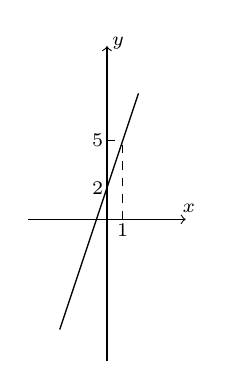
\begin{tikzpicture}[scale=0.2]
\tikzset {line01/.style={line width =0.5pt}}
\tikzset{line02/.style={line width =1pt}}
\tikzset{line03/.style={dashed,line width =0.5pt}}
%\filldraw [black] (0,0) circle (1pt);
\draw [->] (-5,0) -- (5,0);
\draw [->] (0,-9) -- (0,11);
\draw[line01] (-3,-7) -- (2,8);
\draw[line03] (1,0) -- (1,5);
\draw[line03] (0,5) -- (1,5);
\draw (5.2,0.7) node {\scriptsize $x$};
\draw (-0.6,2) node {\scriptsize $2$};
\draw (-0.6,5) node {\scriptsize $5$};
\draw (1,-0.7) node {\scriptsize $1$};
\draw (0.7,11.2) node {\scriptsize $y$};
\end{tikzpicture}$$
б) Эта прямая при любом $a$ проходит через точку $(0;2),$ то есть один из катетов отсекаемого прямоугольного треугольника равен 2. Если второй катет отличается от него в 1,5 раз, то возможны 4 случая: он больше в 1,5 раза и точка пересечения с осью абсцисс имеет положительное или отрицательное значение или он меньше в 1,5 раза и точка пересечения с осью абсцисс имеет положительное или отрицательное значение. Таким образом, искомая прямая должна проходить через одну из точек $(3;0),\ (-3;0),\ \left(\cfrac{4}{3};0\right),\ \left(-\cfrac{4}{3};0\right).$ Подставим эти точки в уравнение прямой и найдём все возможные значения $k:\ 3a+2=0,\ a=-\cfrac{2}{3};\ -3a+2=0,\ a=\cfrac{2}{3};\ \cfrac{4}{3}a+2=0,\ a=-\cfrac{3}{2};\ -\cfrac{4}{3}a+2=0,\ a=\cfrac{3}{2}.$\\
